\chapter{Figures, tables, enumerate and itemize}

%%%%%%%%%%%%%%%%%%%%%%%%%%%%%%%%%%%%%%%%%%%%%%%%%%%%%%%%%%%
%%%%%%%%%%%%%%%%%%%%%%%%%%%%%%%%%%%%%%%%%%%%%%%%%%%%%%%%%%%

\section{Figures}

In almost every document figures will be needed in order to explain a concept or just present something. The package \imp{graphicx} is needed for embedding figures.

\begin{figure}[!h]
	\centering
	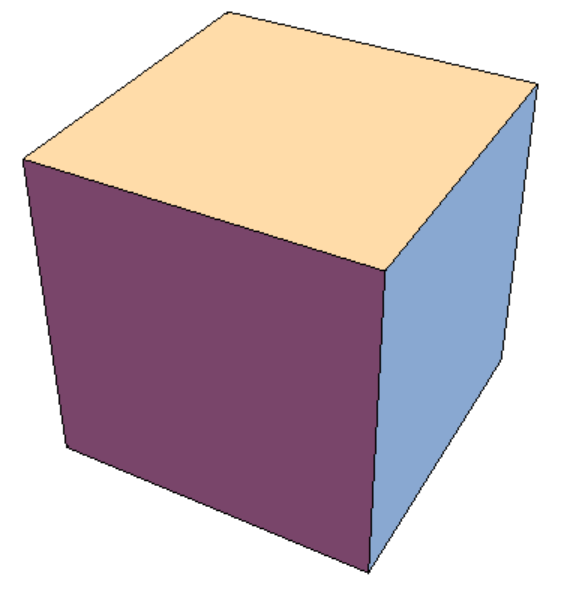
\includegraphics[width=0.3\textwidth]{figures/cube}
	\caption{A figure caption beneath the figure for description of the depicted concept which sometimes can be very long}
	\label{ft_fig_firstfig}
\end{figure}

In \autoref{ft_fig_firstfig}, for example, a PNG image is depicted (compiled with pdflatex). Alternatively, EPS figures can be embedded if dvips and ps2pdf compilation is used. All figures are listed in list of figures with the command \imp{listoffigures}.

%%%%%%%%%%%%%%%%%%%%%%%%%%%%%%%%%%%%%%%%%%%%%%%%%%%%%%%%%%%
%%%%%%%%%%%%%%%%%%%%%%%%%%%%%%%%%%%%%%%%%%%%%%%%%%%%%%%%%%%

\section{Tables}

Data can be presented in tables, e.g., as shown in \autoref{ft_tab_ex}.

\begin{table}[!h]
	\centering
	\begin{tabular}{l|cl}
	\hline \hline
	
		& Property 1
		& Property 2\\ \hline
	Criterion 1
		& 764
		& 23546 \\
	Criterion 2
		& 3
		& 34 \\
	\hline \hline
	\end{tabular}
	\caption{Exemplary table}
	\label{ft_tab_ex}
\end{table}

Sometimes very long tables must be presented which may also go over pages. For this cases the packages \imp{longtable} is useful, as used in 

\begin{center}
\begin{longtable}{l|l|l}

% \baselinestretch{1.5}

 \hline \hline
 $i^3$ & $2i^3$ & $3i^3$ \bigstrut \\ \hline
 \endfirsthead
 
 \multicolumn{3}{c}{\tablename\ \thetable{} -- information message on top} \\
 \hline
 $i^3$ & $2i^3$ & $3i^3$ \bigstrut \\ \hline 
 \endhead
 
 \hline
 \multicolumn{3}{c}{Foot information} \\ \hline
 \endfoot
 
 \hline \hline
 \caption{Long Table}
 \label{lt}
 \endlastfoot
 
 1 & 2 & 3 \\
 8 & 16 & 24 \\
 27 & 54 & 81 \\
 64 & 128 & 192 \\
 125 & 250 & 375 \\
 216 & 432 & 648 \\
 343 & 686 & 1029 \\
 512 & 1024 & 1536 \\
 729 & 1458 & 2187 \\
 1000 & 2000 & 3000 \\
 1331 & 2662 & 3993 \\
 1728 & 3456 & 5184 \\
 2197 & 4394 & 6591 \\
 2744 & 5488 & 8232 \\
 3375 & 6750 & 10125 \\
 4096 & 8192 & 12288 \\
 4913 & 9826 & 14739 \\
 5832 & 11664 & 17496 \\
 6859 & 13718 & 20577 \\
 8000 & 16000 & 24000 \\
 9261 & 18522 & 27783 \\
 10648 & 21296 & 31944 \\
 12167 & 24334 & 36501 \\
 13824 & 27648 & 41472 \\
 15625 & 31250 & 46875 \\
 17576 & 35152 & 52728 \\
 19683 & 39366 & 59049 \\
 21952 & 43904 & 65856 \\
 24389 & 48778 & 73167 \\
 27000 & 54000 & 81000 \\
 29791 & 59582 & 89373 \\
 32768 & 65536 & 98304 \\
 35937 & 71874 & 107811 \\
 39304 & 78608 & 117912 \\
 42875 & 85750 & 128625 \\
 46656 & 93312 & 139968 \\
 50653 & 101306 & 151959 \\
 54872 & 109744 & 164616 \\
 59319 & 118638 & 177957 \\
 64000 & 128000 & 192000 \\
 68921 & 137842 & 206763 \\
 74088 & 148176 & 222264 \\
 79507 & 159014 & 238521 \\
 85184 & 170368 & 255552 \\
 91125 & 182250 & 273375 \\
 97336 & 194672 & 292008 \\
 103823 & 207646 & 311469 \\
 110592 & 221184 & 331776 \\
 117649 & 235298 & 352947 \\
 125000 & 250000 & 375000 \\
\end{longtable}
\end{center}

All tables are listed with \imp{listoftables}.

%%%%%%%%%%%%%%%%%%%%%%%%%%%%%%%%%%%%%%%%%%%%%%%%%%%%%%%%%%%
%%%%%%%%%%%%%%%%%%%%%%%%%%%%%%%%%%%%%%%%%%%%%%%%%%%%%%%%%%%

\section{Enumerate and itemize}

If important sequential points are to presented the environment \imp{enumerate} can be used as follows:
\begin{enumerate}
\item
	Some important stuff
\item
	More stuff
\end{enumerate}
With the package \imp{enumerate} some options can be used, e.g.,
\begin{enumerate}[a)]
\item
	Some important stuff
\item
	More stuff
\end{enumerate}
or 
\begin{enumerate}[~~~1)]
\item
	Some important stuff
\item
	More stuff
\end{enumerate}

Alternatively, point can be just presented without any enumeration with the environment \imp{itemize}
\begin{itemize}
\item
	Some important stuff
\item
	More stuff
\end{itemize}